\chapter{Datenbeschaffung und Speicherung}\label{ch:data}

\section{Ausgangslage}

\section{Die ARD-Audiothek}

Die Podcastbranche wächst seit vielen Jahren stetig und immer mehr Menschen hören regelmäßig Podcasts.
In Deutschland ist die ARD-Audiothek einer der gößten Podcastanbieter mit mitlerweile über 41 Millionen Audioabrufen und über 100.000 verschiedenen Audioinhalten zum Abrufen. 
Im Appstore und im Google Playstore hat die App der Ard Audiothek jeweils über eine Million downloads.
\cite{gotting2023}
Die ARD Audiothek wird von den Landesrundfunkanstalten der ARD und dem Deutschlandradio betrieben und stellt alle deren Audioinhalte zur Verfügung.
Es gibt über 2000 verschiedene Podcasts, in vielen unterschiedlichen Kategorien, wie Comedy, Sport, Wissenschaft,Wirtschaft, Gesellschaft, Kunst, Musik oder Philosophie.
Außerdem gibt es Hörbücher, Hörspiele, oder Podcasts nur für Kinder.
Die einzelnen Rundfunkanstalten tragen außerdem eigene Podcasts bei, die meißt einen regionalen Kontext haben, wie zum Beispiel der Podcast "Giga Grünheide" über das Teslawerk in Brandenburg vom rbb.
Alle diese Inhalte sind kostenlos und frei verfügbar und geben eine gute Quelle für das Audiomaterial ab, welches in dieser Arbeit verwendet wird.



\section{Podcastreihe Radiowissen}

Zur automatischen Generierung von Podcast Episoden bietet es sich an, dass in den Ausgangsaudios die Sprache klar und verständlich ist und verschiedene Sprecher sich nicht ins Wort fallen und gleichzeitig reden.
Außerdem ist es wünschenswerte die ausgeschnittenen Audiosegmente an klaren Satzgrenzen zu teilen, sodass der Ausschnitt nicht mitten im Satz beginnt und dem/der Zuhörer*in der Kontext vorenthalten wird. 

Als Datengrundlage wird die Podcastreihe Radiowissen von bayern2 benutzt. 
Diese ist nicht wie ein klassischer Podcast im Dialogstil aufgebaut, sondern ähnlich wie ein Höhrspiel von einem Manuskript abgelesen.
Dazu kommen verschiedene Geräusche und verschiedene Stimmen, um dem/der Hörer*in mehr Abwechselung zu ermöglichen.

Der Fokus der einzelnen Episoden liegt auf interessanten Beiträgen zu speziellen Themen, die häufig  Themen über Geschichte, Naturwissenschaft, Gesellschaft oder Phillosophie umfasst.
Beispielepisoden sind: "Fasten - Verzicht und innerer Gewinn?", "Die Maus - Anpassungskünstler und gefürchteter Schädling", oder "Maria Sibylla Merian - Naturforscherin und Künstlerin".

Die mehr als 2000 Episoden wurden von mehr als 150 verschiedenen Autoren geskriptet.
Dadurch sind die einzelnen Episoden unterschiedlich in der erzählweise.
In einigen Episoden kommen originale Audiospuren von historischen Aufnahmen vor, oder Gastbeiträge von Experten.
Außerdem wird beinahe jeder Podcast abwechselnd von mehreren Stimmen vorgetragen, was nachweislich die Aufmerksamkeit von Zuhörer*innen verbessert \cite{kang2012}.




\section{Die ARD-Audiothek API}

Die Inhalte in der ARD Audiothek kann man entweder direkt über die die Webseite erreichen, oder mithilfe einer frei benutzbare Web-GraphQL API abfragen.
(https://api.ardaudiothek.de/graphql) 
Über diese Schnittstelle bekommt man alle Informationen, wie den Titel, die Beschreibungen, die Autoren und auch den Link zu dem MP3 File jeder Episode.

Über die GraphQL Abfrage \autoref{ch:graphql-1} erhält man alle Download Links zu den Podcast Episoden des Podcasts "Radio Wissen" von bayern2.
Das sind (Stand 3. Januar 24) 2257 Podcast Episoden.
Dabei kommt es insgesamt 15 mal vor, dass zwei Episoden den selben Titel tragen, aber eine unterschiedliche Download-URL aufweisen.
Die URL unterscheidet sich nur, indem hinten die Zeichen "-1" oder "-2" angefügt wurden.
Zum Beispiel hat die Episode "Quantenphysik - Wahr, aber verrückt" den Downloadlink https://media.neuland.br.de/file/1804047/c/feed/quantenphysik-wahr-aber-verrueckt.mp3 aber auch https://media.neuland.br.de/file/2069613/c/feed/quantenphysik-wahr-aber-verrueckt-1.mp3.
In diesem Fall liefert nur die zweite URL einen Download, die erste zeigt eine Fehlermeldung an.
Es gibt auch Fälle in denen beide Links funktionieren, wie zum Beispiel 
https://media.neuland.br.de/file/32891/c/feed/die-bamberger-hexenprozesse-unschuldig-muss-ich-sterben.mp3 und
https://media.neuland.br.de/file/1858845/c/feed/die-bamberger-hexenprozesse-unschuldig-muss-ich-sterben-1.mp3   

Über eine weitere Anfrage \autoref{ch:graphql-2} bekommt man die Beschreibungen der einzelnen Episoden. 

Jede dieser Episoden ist eine MP3 Datei, von ungefähr 20 Minuten länge und verbraucht ca. 20 MB Speicherplatz.
Zusammen sind diese Audiodaten ungefähr 47 GB groß. 

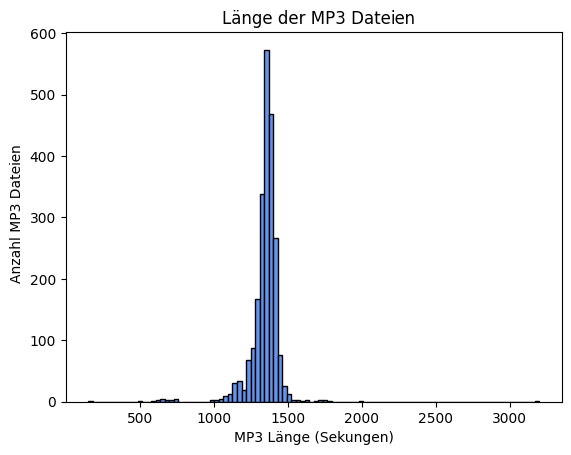
\includegraphics[width=\linewidth]{figures/mp3_length.png}

Der kürzeste Podcast ist "ab-jetzt-in-der-ard-audiothek-kinder-der-flucht-frauen-erzaehlen.mp3", der nur 2 Minuten 30 Sekunden lang ist und ein Teaser für einen anderen Podcast darstellt.
Die längste MP3 Datei ist mit Abstand "deportation-und-exil-eine-polnische-odyssee-im-zweiten-weltkrieg.mp3" mit einer Länge von mehr als 53 Minuten.
Diese Episode ist mehr als doppelt so lang wie eine durchschnittliche Episode (22 Min) und bildet einen Ausnahmefall.


Über die API kann auch in einigen Fällen direkt ein Transkript des Audiofiles angefordert werden. 
Allerdings ist die Transkription meist nicht sehr akkurat.
Nähreres dazu in Kapitel \autoref{ch:method}

\section{Datenspeicherung}

\subsection{Datenspeicherung SQLite}

Die MP3 Datein der einzelnen Podcast Episoden werden in einem seperaten Ordner gespeichert und die Benennung der originalen Datein wird aus der URL übernommen.
Für die Speicherung der Transkripte, wird das relationale Datenbank Managment System (RDBMS) SQLite  genutzt.
SQLite ist für Datenanalysezwecke sehr gut geeignet, weil es simpel und performant ist und das Projekt opensource und kostenlos nutzbar ist.
Im Gegensatz zu anderen RDBMS, wie mySQL oder PostgreSQL arbeitet SQLite Serverlos und speichert alle Tabellen in einer einzigen Datei, was sehr nützlich für den Datenaustausch zwischen verschiedenen Geräten ist.
Für einige Operationen, wie die Transkription der Audiodatein, oder die Generierung von Embeddings wird die Hardware eines High-Performance Clusters der Technischen Hochschule Nürnberg genutzt. 
Um die Daten zu analysieren und zu nutzen bietet es sich an auf Consumer-hardware zu wechseln und dafür ist eine gute Portabilität der Datenbank von Vorteil.

SQLite unterstützt Datenmengen bis zu 140 TB, allerdings auf der offiziellen Webseite angegeben, dass ab einer größe über 1 TB auf serverbasierte RDBMS umgestiegen werden sollte, da die Gesammte Datenbank in einem File gespeichert ist und viele Betriebssysteme eine maximale Größe der Datein vorgeben.
Falls das Projekt in der Zukunft auf mehr Audiomaterial ausgeweitet wird sollte ein Wechsel des DBMS in betracht gezogen werden.

\subsection{Datenspeicherung Vektoren SQLite}

Da SQlite nativ keine Listen oder Tabellen als Einträge in einer Datenbank speichern kann, ist es nicht trivial, die Embeddings abzuspeichern.
Zunächst wurde die Möglichkeit in betracht gezogen, jeden einzelnen Eintrag aus einem Embedding als seperaten Eintrag in einer Tabelle zu speichern. 

Das führt allerdings zu sehr ineffizienten Abfragen der Daten und beim Einfügen von Daten limitiert SQLite die Anzahl der parameter, sodass längere Embeddings umständlich gestückelt abgespeichert werden müssten.

Als nächstes wurde überprüft, ob man jedes Embedding als Serialisiertes Array abspeichern kann.
Dafür wurde jedes Embedding in einen JSON String umgewandelt, um diesen abzuspeichern. 
Dabei kommt leider das Problem auf, dass die Daten bei der Verwendung wieder deserialisiert werden müssen.
Dieser Schritt müsste jedes mal wiederholt werden, wenn eine Suche stattfindet und dauert sehr lange und ist sehr ineffizient. 
Auf den 400.000 Sätzen mit einem 384 dimensionalen Embedding eines Sentence Transformer Modells ca. 45 Min.


\subsection{Datenspeicherung Dense Vektoren}

Um Dichte Vektoren abzuspeichern, bietet es sich an eine seperate Vektordatenbank an.
Eine Vektordatenbank ist eine nichtrelationale Datenbank, die darauf spezialisiert ist, ungeordnete Informationen zu ordnen.
Dazu speichert sie die Embeddingvektoren verschiedener Datenquellen effizient ab und erlaubt Zugriff auf schnelle Suchalgorithmen, wie Approximate Nearest Neighbour Algorithmen.

Es gibt verschiedene Approximate Nearest Neighbour Algorithmen, die alle darauf abzielen, den gesamten Suchraum für eine Ähnlichkeitssuche in kleinere Unterräume aufzuteilen.
Dabei werden oft Baum Strukturen verwendet, um die Suche effizienter zu gestalten.
Speziell Algorithmen wie Hierarchical Navigable Small Worlds werden von vielen Vektordatenbanken benutzt.

Vektordatenbanken entwickeln sich in den letzten Jahren stark weiter.
Bekannte Vektordatenbanken sind zum Beispiel Milvus, die sehr gut auf große Datenmengen skalieren kann und deshalb in vielen großen Unternehmen, wie Nvidia, Paypal oder ebay benutzt.
Milvus bietet Unterstützung für eine Clusterbasierte Struktur, in der einzelne Container dynamisch zusammenarbeiten können.
Dadurch wird eine hohe skalierbarkeit auf große Datenmengen erreicht, für kleinere Projekte ist der Setup Aufwand sehr groß und die Lernkurve sehr Steil.

Pinecone, Zilliz, Qdrant

Außerdem gibt es eine erweiterung für die PostGreSQL Datenbank namens pg-Vector

Die Vektordatenbank Redis

Durch die Neuheit der Vektordatenbanken bedingt, gibt es kaum Vergleiche zwischen diesen.
\cite{blueteamai}


% In dieser Arbeit wird die Vektordatenbank Milvus verwendet.
% Milvus ist eine Open-Source Vektordatenbank die von dem Unternehmen Zilliz entwickelt wird.
% Laut eigenen Angaben ist sie die am weitseten fortgeschrittene Vektordatenbank und wird von vielen Unternehmen, wie Nvidia, Paypal oder ebay benutzt.

In dieser Arbeit wird die Vektordatenbank Chroma verwendet. 
Chroma ist eine einfache Vektordatenbank, die die Daten entweder lokal, oder über eine client-server Schnittstelle speichern kann.
Das Projekt ist erst im Mai 2022 als Startup entstanden, verfügt aber mittlerweile über viele Features, die die Datenverwaltung erheblich vereinfachen.
Die Datenbank ist dabei mit einer NoSQL Datenbank zu vergleichen, indem die Daten nicht relational in Tabellen gespeichert werden, sondern in einer Collection als Objekte mit verschiedenen Metadaten.
Jedes dieser Objekte hat eine Document Eigenschaft, welche den Inhalt des Dokuments repräsentiert.
Dieser Inhalt ist in diesem Fall ein Ausschnitt aus einem Transkript, könnte aber auch ein Bild oder eine Audiodatei darstellen.
Außerdem hat jedes Objekt ein Embeddingvektor, der mit dem Dokument assoziiert wird. 
Innerhalb einer Collection müssen alle Objekte mit der selben Embeddingmethode encodiert werden.
Das sichert die Vergleichbarkeit der verschiedenen Vektoren untereinander.
ChromaDB bietet nativen support für verschiedene Embedding Modelle von OpenAI, Huggingface, Cohere, instructorembedding und JinaAI.
Dafür müssen nur das Model und der Plattformspezifische API-KEY angegeben werden und Chroma erstellt automatisch für jedes Dokument das Embedding.
Alternativ können auch schon vorgefertigte Embeddings eingefügt und die dazugehörige Embedding Funktion eingetragen werden.
Standartmäßig ist das Embedding des Sentence Transformer Modells all-MiniLM-L6-v2 eingestellt.

Chroma bietet außerdem sehr guten Support für effizientes Retrieval von Dokumenten.
 


In deisem Projekt wurde erst in einer späten Phase der Umstieg auf die Vektor-datenbank vollzogen, weshalb einige Funktionen, die diese Datenbank automatisch integriert hat noch einmal sehr ausführlich beschrieben werden.




\subsection{Datenspeicherung Sparce Vektoren}

Chroma bietet leider noch keine Unterstützung zur speicherung von Sparce Vektoren
Stattdessen wurde das python Modul pickle verwendet, welches arauf spezialisiert ist, python Objekte effizient als bytecode zu serialisieren. 
Es bietet auch die Möglichkeit Datenstrukturen effizient zu speichern und zu laden und hat seit Python 3.8 auch guten support, um große NumPy Arrays effizient zu speichern, was zuvor nur mit der joblib Bibliothek möglich war.
Pickle speichert die Daten in einem Python spezifischen Format ab, was zwar schlecht für die Portierbarkeit auf andere Systeme ist, es aber erlaubt verschiedene Eigenschaften besser zu speichern als JSON (Zum Beispiel Pointer sharing).

Für den TF-IDF Algorithmus, bei dem ein Vokabular von mehr als 200.000 Wörtern eine ebensogroße Dimensionalität der Embeddingvektoren benötigt, würde ein normaler Serialisierungsalgorithmus für die 300.000 Sätze ca 60 Milliarden Werte abspeichern.
Wenn man für jeden dieser Werte eine 32 Bit Gleitkommazahl als Datentyp abspeichern würde, käme man auf ca. 240 GB Daten. 
Ein großteil dieser Werte (~99,9\%) sind dabei 0.
Ein Numpy Array kann diese Werte sehr effizient zusammenfassen und mithilfe von pickle kann dieses kompakte Array effizient abgespeichert werden, was in einer tatsächlichen Größe von ca. 50 MB entspricht.

\subsection{weitere Schritte}


Eine bekannte Bibliothek für Nearest Neighbour Searches ist Annoy, die unter anderem bei Spotify für die Recommendations von Songs verwendet wird. [Quelle]
Eine weitere bekannte bekannte Bibliothek für Nearest Neighbour Searches ist FAISS (Facebook AI Similarity Search)

